\documentclass[12pt]{article}
\usepackage{graphicx}

\usepackage{amsmath}
\usepackage{amsfonts}
\usepackage{graphicx}
\usepackage{geometry}
\graphicspath{ {./imgs/plots/}{./imgs/graphs/} }
\geometry{margin=4cm}

\title{Relazione progetto di Calcolo Numerico\\ A.A. 2021/2022}
\author{Apollonio Francesco\\Bianchi Andrea\\Mazzetti Francesca}

\begin{document}

\begin{titlepage}
\maketitle
\pagenumbering{gobble}
\end{titlepage}
\newpage
\tableofcontents
\newpage
\pagenumbering{arabic}

\section{Introduzione}

    Il problema di Deblur consiste nella ricostruzione di un'immagine a partire da un dato acquisito mediante il modello:
    \begin{align*}
        b = Ax + \eta
    \end{align*}
    Con $b$ che è l'immagine corrotta, $x$ l'immagine originale da ricostruire, la matrice $A$ applica il blur gaussiano e $\eta$ è il rumore aggiunto all'immagine sfocata, con distribuzione Gaussiana di media $\mathbb{O}$ e deviazione standard $\sigma$.

    \subsection{Il dataset}
    Per eseguire i test richiesti è stato generato un dataset di otto immagini contenenti forme geometriche varie su sfondo nero a cui sono state aggiunte due ulteriori immagini fotografiche, delle quali una, la figura "sample9.png" molto contrastata e con pochi dettagli e l'altra, "sample10.png" meno contrastata ma più dettagliata.

    \subsection{Gli algoritmi}
    Per ricostruire le immagini danneggiate sono stati impiegati diversi algoritmi, in modo da poter poi confrontarne l'efficacia.

    \paragraph{La soluzione naive}
    Il primo tentativo di ricostruzione è stato fatto utilizzando un algoritmo semplice - per questo detto naive - per risolvere il problema di ottimizzazione:
    \begin{align*}
        x^* = \arg\min_x \frac{1}{2} ||Ax - b||_2^2
    \end{align*}
    In questo caso la funzione da minimizzare è $f(x) = \frac{1}{2} ||Ax - b||_2^2$ e il suo gradiente è $\nabla f(x) = A^TAx - A^Tb$. La funzione è stata implementata usando il metodo dei gradienti coniugati, implementato dalla funzione minimize inclusa nella libreria numpy.

    \paragraph{Regolarizzazione}
    Dal momento che la funzione naive recupera sì la nitidezza dell'immagine, ma introduce un rumore elevato, è necessario introdurre un termine di regolarizzazione di Tikhonov, il problema di minimizzazione diventa quindi:
    \begin{align*}
        x^* = \arg\min_x \frac{1}{2} ||Ax - b||_2^2 + \frac{\lambda}{2} ||x||_2^2
    \end{align*}
    La funzione da minimizzare è quindi $f(x) = \frac{1}{2} ||Ax - b||_2^2 + \frac{\lambda}{2} ||x||_2^2$ e il suo gradiente è $\nabla f(x) = A^TAx - A^Tb + \lambda x$.
    La funzione è stata implementata sia tramite la funzione minimize inclusa nella libreria numpy che tramite il metodo del gradiente illustratoci a lezione. Sono poi stati eseguiti test con diversi valori di lambda.

    \paragraph{Variazione totale}
    Un altro termine di regolarizzazione adatto è dato dalla funzione di Variazione Totale. Data $x$ l'immagine di dimensioni $n\times m$, la variazione totale $TV$ di $x$ è definita come:
    \begin{align*}
        TV(u) = \sum_i^n{\sum_j^m{\sqrt{||\nabla u(i, j)||_2^2 + \epsilon^2}}}
    \end{align*}
    Il problema di minimo da risolvere diventa quindi:
    \begin{align*}
        x^* = \arg\min_x \frac{1}{2} ||Ax - b||_2^2 + \lambda TV(u)
    \end{align*}
    il cui gradiente è:
    \begin{align*}
    \nabla f(x) = (A^TAx - A^Tb)  + \lambda \nabla TV(x)
    \end{align*}
    La funzione è stata implementata usando il metodo del gradiente visto a lezione e già utilizzato nel precedente punto. Sono stati eseguiti test per diversi valori di $\lambda$.

    \subsection{I test}
    Dopo aver applicato il blur gaussiano e il disturbo alle immagini del dataset, abbiamo applicato diversi algoritmi per migliorare la qualità delle immagini. Per ogni immagine abbiamo eseguito un ciclo di test applicando diversi blur gaussiani, diversi valori di deviazione standard per il rumore e diversi valori per il parametro $\lambda$ del termine di regolarizzazione di Tikhonov. In tutti i test i metodi sono stati limitati ad un numero massimo di iterazioni pari a 100, per permettere di elaborare tutte e dieci le immagini in un tempo ragionevole. I valori usati sono riassunti nella tabella 1.

    \medskip
    \begin{table}[htb]
    \centering
    \begin{tabular}{||c c c c||}
         \hline
         Dim Kernel & Std dev Sigma Kernel & Std Dev Rumore & Lambda \\ [0.5ex]
         \hline\hline
         5 $\times$ 5 & 0.5 & 0.01 & 0.01 \\
         \hline
         7 $\times$ 7 & 1 & 0.02 & 0.05 \\
         \hline
         9 $\times$ 9 & 1.3 & 0.03 & 0.08 \\
         \hline
         N.A. & N.A. & 0.04 & 0.32 \\
         \hline
         N.A. & N.A. & 0.05 & 1 \\ [0.2ex]
         \hline
    \end{tabular}
    \caption{Valori assunti dai parametri nei test}
    \label{table:1}
    \end{table}

    I dati raccolti possono essere trovati integralmente nella cartella "data" allegata, di seguito commenteremo i risultati più rilevanti.

\section{Analisi dei risultati ottenuti}
    Dai test effettuati sulle immagini (di seguito riporteremo solo due delle dieci immagini elaborate; le restanti immagini possono essere trovate nella galleria a fine documento) possiamo immediatamente notare come la correzione naive risulti largamente insufficiente ai fini di una ricostruzione accurata della figura di partenza.

    I due metodi regolarizzati con parametro di Tikhonov danno risultati ottimi e simili fra loro. Il metodo del gradiente regolarizzato con parametro $TV$ offre, invece, un risultato migliore nel caso di immagini con forme geometriche astratte ma genera figure non del tutto nitide (quasi come se fosse un effetto "acquerello") nel caso di scatti fotografici.

    Ricordiamo, comunque, che dal momento che i metodi utilizzati sono iterativi, le funzioni convergenti e che, nel caso dei nostri test, i metodi sono stati limitati a 100 iterazioni, possiamo aspettarci un aumento della qualità del miglioramento con l'aumentare del numero di iterazioni.

    \newpage
    \begin{figure}[h!]
    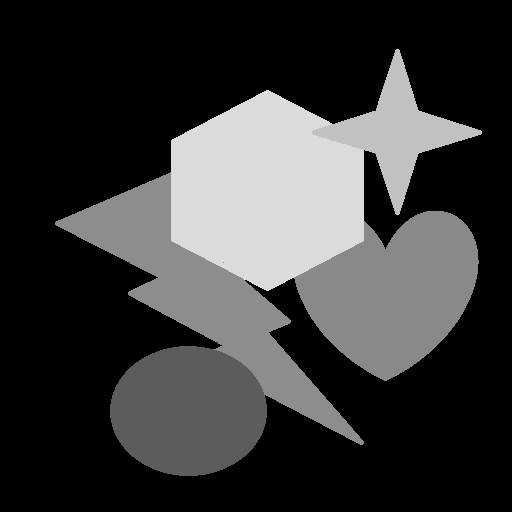
\includegraphics[width=14cm]{sample5}
    \caption{sample5.png - Dim. Kernel: $9\times9$, $\sigma:1.3$,Std. Dev.:$0.05$, $\lambda:0.08$}
    \end{figure}
    \newpage
    \begin{figure}[h!]
    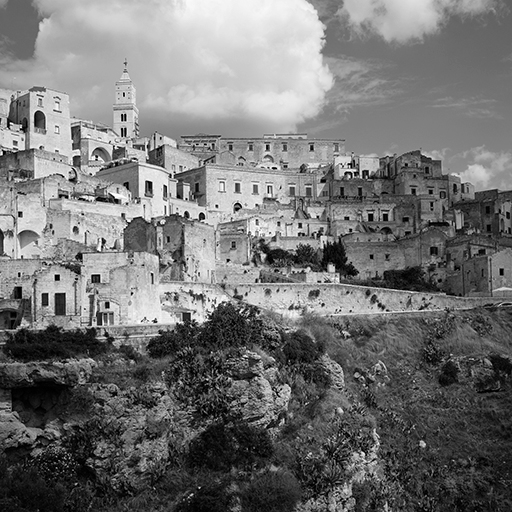
\includegraphics[width=14cm]{sample10}
    \caption{sample10.png - Dim. Kernel: $9\times9$, $\sigma:1.3$,Std. Dev.:$0.05$, $\lambda:0.08$}
    \end{figure}
    \newpage

\section{PSNR e MSE al variare dei parametri}
\subsection{Introduzione}
    Nel fare i test volti al raccoglimento dei dati sulla vairiazione di PSNR e MSE, abbiamo alterato la dimensione del kernel, il valore di $\sigma$, la deviazione standard del rumore e il valore del parametro di regolarizzazione usando i valori riportati nella tabella \ref{table:1}. Abbiamo così ottenuto 75 differenti valori di PSNR ed MSE per ogni algoritmo applicato su un immagine, per un totale di 750 valori per l'intero dataset. Dato che una tabella di simili dimensioni richiederebbe troppo spazio all'interno di questo documento, riportiamo in questa sede solo le tabelle con le medie dei valori ottenuti fra le 10 immagini di alcuni test scelti. Per i dati completi rimandiamo ai file .csv allegati.
    I parametri sono indicati con la notazione KX\_Y\_Z; dove X indica la dimensione e il valore di sigma del kernel (K1 equivale ad un kernel di dimensione $5\times5$ con valore di $\sigma=0.5$, K2 equivale ad una dimensione di $7\times7$ con $\sigma=1$ e K3 indica un kernel di dimensione $9\times9$ con $\sigma=1.3$), Y indica il valore della deviazione standard del rumore e Z il valore del parametro $\lambda$.

    \subsection{Variazione del PSNR}
    \begin{table}[!ht]
    \centering
    \begin{tabular}{|l|l|l|l|l|l|}
    \hline
        Parametri & Noised & Naive & Tikhonov1 & Tikhonov2 & TV \\ \hline
        K1\_0.01\_0.01 & 32.888 & 20.906 & 28.853 & 29.397 & 40.310 \\ \hline
        K1\_0.02\_0.05 & 30.763 & 14.891 & 27.670 & 27.671 & 36.089 \\ \hline
        K1\_0.03\_0.08 & 28.663 & 11.362 & 25.762 & 25.762 & 34.484 \\ \hline
        K1\_0.04\_0.32 & 26.830 & 8.861 & 21.422 & 21.422 & 30.933 \\ \hline
        K1\_0.05\_1 & 25.248 & 6.925  & 15.829 & 15.829 & 26.091 \\ \hline
        K2\_0.01\_0.01 & 30.625 & 8.963 & 29.434 & 30.134 & 36.806 \\ \hline
        K2\_0.02\_0.05 & 29.216 & 2.883 & 28.629 & 28.630 & 33.337 \\ \hline
        K2\_0.03\_0.08 & 27.613 & -0.660 & 26.921 & 26.921 & 32.157 \\ \hline
        K2\_0.04\_0.32 & 26.084 & -3.171 & 21.414 & 21.414 & 29.549 \\ \hline
        K2\_0.05\_1 & 24.697 & -5.128 & 15.785 & 15.785 & 26.568 \\ \hline
        K3\_0.01\_0.01 & 29.929 & 9.127 & 29.723 & 30.262 & 35.828 \\ \hline
        K3\_0.02\_0.05 & 28.696 & 3.018 & 28.697 & 28.699 & 32.249 \\ \hline
        K3\_0.03\_0.08 & 27.238 & -0.550 & 27.071 & 27.071 & 31.340 \\ \hline
        K3\_0.04\_1 & 25.812 & -3.069 & 15.764 & 15.764 & 26.297 \\ \hline
        K3\_0.05\_1 & 24.497 & -5.031 & 15.759 & 15.759 & 26.284 \\ \hline
    \end{tabular}
    \caption{PSNR medi in test scelti }
    \label{table:2}
    \end{table}

    \subsection{Variazione del MSE}
    \begin{table}[!ht]
    \centering
    \begin{tabular}{|l|l|l|l|l|l|}
    \hline
        Parametri & Noised & Naive & Tikhonov1 & Tikhonov2 & TV \\ \hline
        K1\_0.01\_0.01 & 0.00062 & 0.0081 & 0.0013 & 0.0011 & 0.00021 \\ \hline
        K1\_0.02\_0.05 & 0.00092 & 0.0324 & 0.0017 & 0.0017 & 0.00059 \\ \hline
        K1\_0.03\_0.08 & 0.00142 & 0.0730 & 0.0027 & 0.0027 & 0.00080 \\ \hline
        K1\_0.04\_0.32 & 0.00211 & 0.1299 & 0.0083 & 0.0083 & 0.00168 \\ \hline
        K1\_0.05\_1    & 0.00302 & 0.2029 & 0.0313 & 0.0313 & 0.00352 \\ \hline
        K2\_0.01\_0.01 & 0.00108 & 0.1269 & 0.0011 & 0.0010 & 0.00049 \\ \hline
        K2\_0.02\_0.05 & 0.00138 & 0.5148 & 0.0014 & 0.0014 & 0.00092 \\ \hline
        K2\_0.03\_0.08 & 0.00188 & 1.1643 & 0.0021 & 0.0021 & 0.00113 \\ \hline
        K2\_0.04\_0.32 & 0.00258 & 2.0757 & 0.0085 & 0.0085 & 0.00198 \\ \hline
        K2\_0.05\_1    & 0.00348 & 3.2576 & 0.0316 & 0.0316 & 0.00334 \\ \hline
        K3\_0.01\_0.01 & 0.00128 & 0.1222 & 0.0011 & 0.0010 & 0.00061 \\ \hline
        K3\_0.02\_0.05 & 0.00158 & 0.4990 & 0.0015 & 0.0015 & 0.00107 \\ \hline
        K3\_0.03\_0.08 & 0.00208 & 1.1352 & 0.0021 & 0.0021 & 0.00127 \\ \hline
        K3\_0.04\_0.32 & 0.00278 & 2.0320 & 0.0086 & 0.0086 & 0.00211 \\ \hline
        K3\_0.05\_1    & 0.00368 & 3.1857 & 0.0318 & 0.0318 & 0.00348 \\ \hline
    \end{tabular}
    \caption{MSE medi in test scelti }
    \label{table:4}
    \end{table}

    \subsection{Analisi dei dati ottenuti}
    L'analisi delle misure di PSNR e MSE va in contrasto con quanto osservato nelle immagini analizzate poc'anzi. Risulta, infatti, che il valore di PSNR dell'algoritmo che implementa il metodo del gradiente con il parametro di regolarizzazione $TV$ sia sempre superiore a quello degli altri algoritmi, nonostante, come già riportato, le immagini fotografiche ottenute con lo stesso metodo risultino, se pur all'apparenza, qualitativamente inferiori (almeno nel caso di un massimo di 100 iterazioni).

\newpage
\section{Medie e Deviazioni standard}
    Abbiamo poi calcolato, per alcuni parametri fissati, i valori medi e la deviazione standard di PSNR e MSE calcolati sull'intero set di immagini, di seguito riportati.

    \subsection{PSNR - Medie}

    \begin{table}[!h]
    \centering
    \begin{tabular}{|l|l|l|l|l|l|}
    \hline
        Parametri & Noised & Naive & Tikhonov1 & Tikhonov2 & TV \\ \hline
        K1\_0.02\_0.32 & 30.763 & 14.894 & 21.781 & 21.781 & 31.042 \\ \hline
        K1\_0.04\_0.08 & 26.828 & 8.878  & 23.923 & 23.923 & 34.110 \\ \hline
        K2\_0.01\_0.05 & 30.622 & 8.966  & 30.553 & 30.553 & 33.510 \\ \hline
        K2\_0.03\_0.01 & 27.612 & -0.671 & 21.223 & 22.298 & 34.238 \\ \hline
        K2\_0.04\_1    & 26.078 & -3.175 & 15.791 & 15.791 & 26.581 \\ \hline
        K3\_0.01\_0.32 & 29.933 & 9.123  & 21.522 & 21.522 & 29.281 \\ \hline
        K3\_0.03\_0.08 & 27.238 & -0.550 & 27.071 & 27.071 & 31.340 \\ \hline
        K3\_0.05\_0.05 & 24.494 & -5.038 & 24.107 & 24.110 & 31.849 \\ \hline
    \end{tabular}
    \caption{PSNR medi}
    \label{table:6}
    \end{table}

    Analizzando tale tabella possiamo notare come le medie rappresentano esattamente i valori che ci aspettavamo: la qualità dell'immagine migliora sensibilmente ed in ogni caso utilizzando la funzione di Variazione Totale. Scarse differenze possiamo invece notare tra i due algoritmi del metodo del gradiente.
    Da notare sono, inoltre, i valori del PSNR negativi per K3 ( Kernel di dimensione 9 x 9 con sigma = 1.3 ). Ciò avviene a causa del Kernel utilizzato: esso rende estremamente costosa computazionalmente la generazione dell'immagine a tal punto da non essere eseguita totalmente. Questo rende tali valori inaffidabili.

    \newpage
    \subsection{PSNR - Deviazioni standard}
    \begin{table}[!ht]
    \centering
    \begin{tabular}{|l|l|l|l|l|l|}
    \hline
        Parametri & Noised & Naive & Tikhonov1 & Tikhonov2 & TV \\ \hline
        K1\_0.02\_0.32 & 1.658 & 0.0236 & 2.641 & 2.641 & 4.471 \\ \hline
        K1\_0.04\_0.08 & 0.841 & 0.0410 & 0.582 & 0.582 & 4.472 \\ \hline
        K2\_0.01\_0.05 & 2.528 & 0.0375 & 2.172 & 2.172 & 4.362 \\ \hline
        K2\_0.03\_0.01 & 1.577 & 0.0192 & 0.168 & 0.233 & 3.687 \\ \hline
        K2\_0.04\_1    & 1.228 & 0.0314 & 2.743 & 2.743 & 3.538 \\ \hline
        K3\_0.01\_0.32 & 2.572 & 0.0794 & 2.637 & 2.637 & 3.872 \\ \hline
        K3\_0.03\_0.08 & 1.697 & 0.0467 & 1.831 & 1.831 & 3.788 \\ \hline
        K3\_0.05\_0.05 & 1.072 & 0.0192 & 0.824 & 0.825 & 3.800 \\ \hline
    \end{tabular}
    \caption{PSNR deviazioni standard}
    \label{table:8}
    \end{table}


    Analizziamo i risultati ottenuti dall'anlisi statistica delle "Deviazioni Standard".
    Notiamo immediatamente come i valori che tendono a discostarsi maggiormente dalla loro media sono i PSNR risultanti dall'utilizzo della funzione di Variazione Totale.
    D'altro canto i risultati più "affidabili mediamente" risultano essere invece quelli del PSNR dell'immagine corrotta.
    In linee generali possiamo infine notare un andamento di tale valore crescente al crescere delle dimensioni del Kernel.

    \newpage
    \subsection{MSE - Medie}

    \begin{table}[!ht]
    \centering
    \begin{tabular}{|l|l|l|l|l|l|}
    \hline
        Parametri & Noised & Naive & Tikhonov1 & Tikhonov2 & TV \\ \hline
        K1\_0.02\_0.32 & 0.00092 & 0.0323 & 0.00790 & 0.00790 & 0.00166 \\ \hline
        K1\_0.04\_0.08 & 0.00212 & 0.1294 & 0.00409 & 0.00409 & 0.00083 \\ \hline
        K2\_0.01\_0.05 & 0.00108 & 0.1268 & 0.00102 & 0.00102 & 0.00091 \\ \hline
        K2\_0.03\_0.01 & 0.00188 & 1.1671 & 0.00755 & 0.00589 & 0.00064 \\ \hline
        K2\_0.04\_1    & 0.00259 & 2.0775 & 0.03167 & 0.03167 & 0.00333 \\ \hline
        K3\_0.01\_0.32 & 0.00128 & 0.1223 & 0.00844 & 0.00844 & 0.00207 \\ \hline
        K3\_0.03\_0.08 & 0.00208 & 1.1352 & 0.00218 & 0.00218 & 0.00127 \\ \hline
        K3\_0.05\_0.05 & 0.00368 & 3.1904 & 0.00396 & 0.00396 & 0.00113 \\ \hline
    \end{tabular}
    \caption{MSE medi }
    \label{table:10}
    \end{table}

    \subsection{MSE - Deviazioni standard}
    \begin{table}[!ht]
    \centering
    \begin{tabular}{|l|l|l|l|l|l|}
    \hline
        Parametri & Noised & Naive & Tikhonov1 & Tikhonov2 & TV \\ \hline
        K1\_0.02\_0.32 & 0.000509 & 0.000175 & 0.004603 & 0.00460 & 0.00274 \\ \hline
        K1\_0.04\_0.08 & 0.000511 & 0.001225 & 0.000590 & 0.00059 & 0.00143 \\ \hline
        K2\_0.01\_0.05 & 0.000989 & 0.001092 & 0.000718 & 0.00071 & 0.00151 \\ \hline
        K2\_0.03\_0.01 & 0.000983 & 0.005180 & 0.000307 & 0.00033 & 0.00095 \\ \hline
        K2\_0.04\_1    & 0.000990 & 0.015020 & 0.018500 & 0.01850 & 0.00385 \\ \hline
        K3\_0.01\_0.32 & 0.001187 & 0.002201 & 0.005215 & 0.00521 & 0.00299 \\ \hline
        K3\_0.03\_0.08 & 0.001185 & 0.012188 & 0.001236 & 0.00123 & 0.00188 \\ \hline
        K3\_0.05\_0.05 & 0.001187 & 0.014144 & 0.000918 & 0.00091 & 0.00167 \\ \hline
    \end{tabular}
    \caption{MSE deviazioni standard}
    \label{table:12}
    \end{table}

    L'analisi statistica dei parametri di MSE ottenuti ci riporta dei risultati estremamente positivi.
    Notiamo infatti come ognuno dei valori in tabella risulti strettamente minore anche di una singola unità: tutti valori MSE risultano estremamente simili tra loro quindi vicini alla loro stessa media.

    \newpage

\section{Analisi delle proprietà dai metodi numerici}
    Analizziamo, infine, l'andamento del metodo del gradiente e del metodo dei gradienti coniugati. Gli algoritmi sono stati eseguiti su due immagini del dataset: l'immagine sample5 (figure geometriche) e l'immagine sample10 (scatto fotografico).
    I dati raccolti sono commentati di seguito.

    \subsection{L'andamento dell'errore}
    I dati raccolti sono stati inseriti nei due grafici (Figura \ref{graph:1} e Figura \ref{graph:2}) qui riportati, il primo si riferisce all'esecuzione sull'immagine sample5 mentre il secondo all'esecuzione sull'immagine sample10.

    Possiamo notare come in entrambe le esecuzioni l'errore del metodo del gradiente varia maggiormente durante le prime iterazioni rispetto a quello del metodo dei gradienti coniugati. Entrambi i metodi però si stabilizzano presso valori simili all'aumentare delle iterazioni

    \begin{figure}[h!]
    \centering
    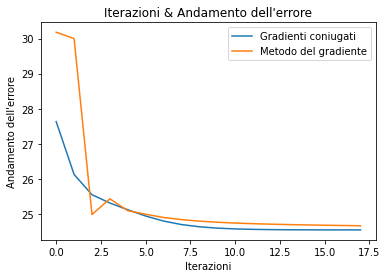
\includegraphics[width=10cm]{sample5-err}
    \caption{Andamento dell'errore, confronto fra parametro di Tikhonov e TV su immagine sample5}
    \label{graph:1}
    \end{figure}

    \begin{figure}[h!]
    \centering
    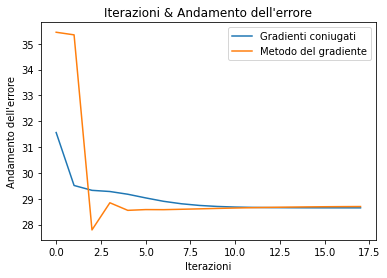
\includegraphics[width=10cm]{sample10-err}
    \caption{Andamento dell'errore, confronto fra parametro di Tikhonov e TV su immagine sample10}
    \label{graph:2}
    \end{figure}

    \newpage
    \subsection{L'andamento della funzione obiettivo}
    Anche in questo caso i dati raccolti sono stati inseriti nei due grafici (Figura \ref{graph:3} e Figura \ref{graph:4}) qui riportati: il primo grafico si riferisce all'esecuzione sull'immagine sample5 mentre il secondo a quella sull'immagine sample10.

    Possiamo notare come in entrambe le esecuzioni l'andamento della funzione usata nel metodo del gradiente è migliore rispetto all'andamento della funzione usata nel metodo dei gradienti coniugati.

    Fin dalle primissime iterazioni, inoltre, la funzione di entrambi i metodi assume un andamento asintotico.
    Questo ci permette di dedurre come un auspicabile miglioramento del risultato,  ottenibile da un aumento delle iterazioni, è in realtà relativamente ridotto; possiamo infatti ottenere delle figure ottimali già con un basso numero di iterazioni.

    \begin{figure}[h!]
    \centering
    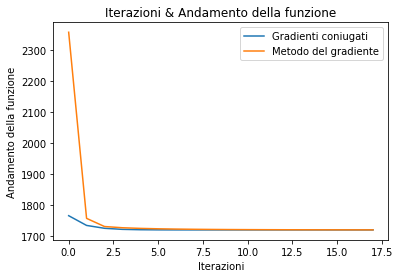
\includegraphics[width=10cm]{sample5-fun}
    \caption{Andamento della funzione, confronto fra parametro di Tikhonov e TV su immagine sample5}
    \label{graph:3}
    \end{figure}

    \begin{figure}[h!]
    \centering
    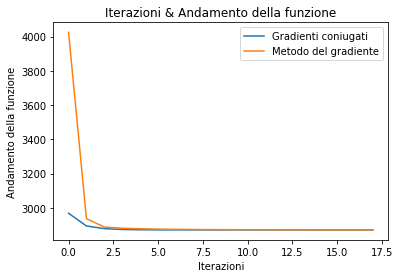
\includegraphics[width=10cm]{sample10-fun}
    \caption{Andamento della funzione, confronto fra parametro di Tikhonov e TV su immagine sample10}
    \label{graph:4}
    \end{figure}

\cleardoublepage

\cleardoublepage
    \subsection{L'andamento della norma del gradiente}
    Analizziamo, infine, l'andamento della norma del gradiente della funzione da minimizzare. Anche in questo caso, come nei precedenti, i dati raccolti sono stati inseriti nei due grafici (Figura \ref{graph:5} e Figura \ref{graph:6}) sotto riportati, il primo grafico si riferisce all'esecuzione sull'immagine sample5 mentre il secondo a quella sull'immagine sample10.

    Possiamo notare come in entrambe le esecuzioni l'andamento della norma gradiente della funzione è pressapoco simile per entrambi i metodi scelti.

    La norma del metodo del gradiente inizialmente è maggiore, ma anche in questo caso è sufficiente superare le prime iterazioni perché il risultato si stabilizzi ed entrambe le implementazioni assumano un andamento simile.

    \begin{figure}[h!]
    \centering
    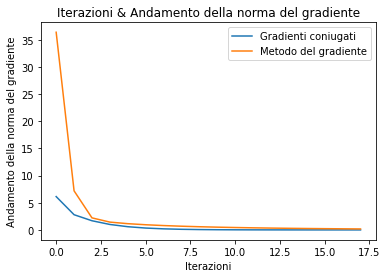
\includegraphics[width=10cm]{sample5-norm}
    \caption{Andamento della norma del gradiente, confronto fra parametro di Tikhonov e TV su immagine sample5}
    \label{graph:5}
    \end{figure}

%
\makeatletter
\setlength{\@fptop}{0pt}
\makeatother
%
    \begin{figure}[t!]
    \centering
    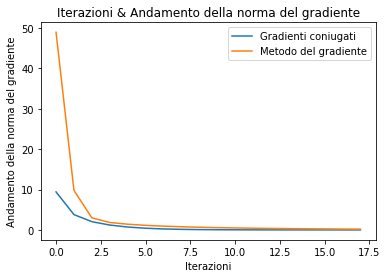
\includegraphics[width=10cm]{sample10-norm}
    \caption{Andamento della norma del gradiente, confronto fra parametro di Tikhonov e TV su immagine sample10}
    \label{graph:6}
    \end{figure}

    \clearpage
    \listoffigures
    \newpage
    \listoftables

\cleardoublepage
    \centering
    \huge
    Galleria
\cleardoublepage

    \begin{figure}[h!]
    \centering
    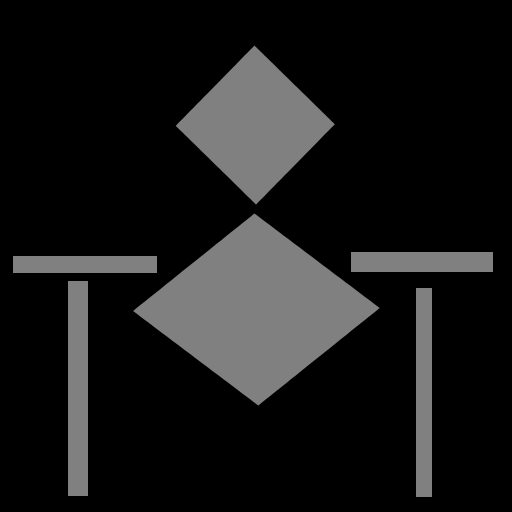
\includegraphics[width=14cm]{sample1}
    \end{figure}
    \newpage

    \begin{figure}[h!]
    \centering
    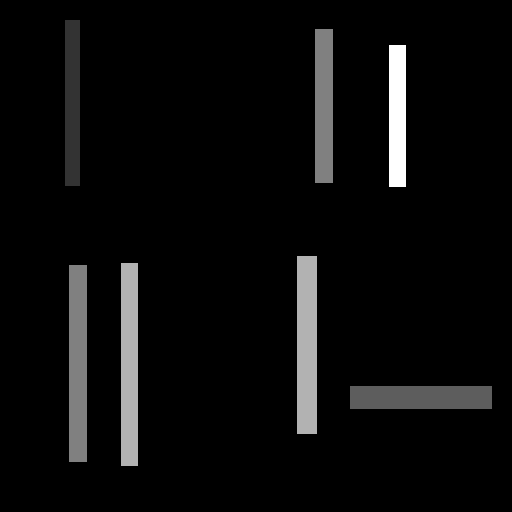
\includegraphics[width=14cm]{sample2}
    \end{figure}
    \newpage

    \begin{figure}[h!]
    \centering
    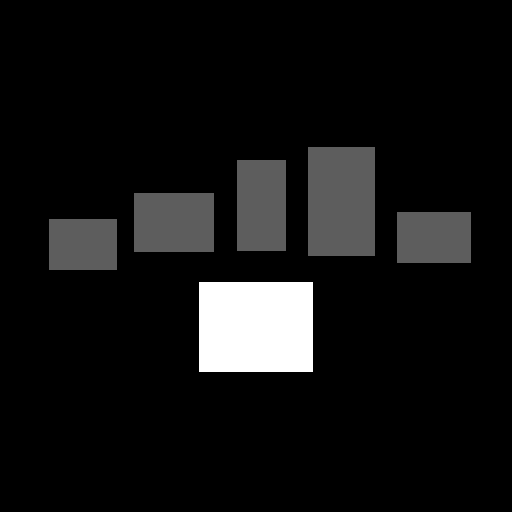
\includegraphics[width=14cm]{sample3}
    \end{figure}
    \newpage

    \begin{figure}[h!]
    \centering
    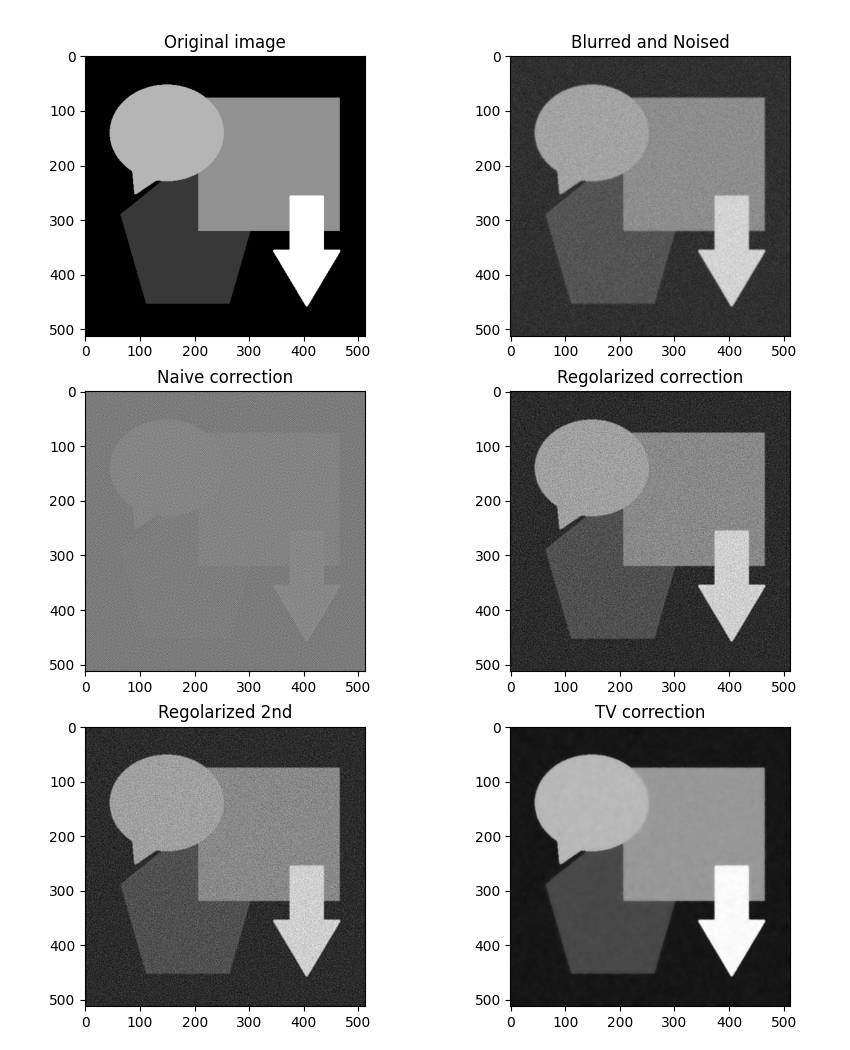
\includegraphics[width=14cm]{sample4}
    \end{figure}
    \newpage

    \begin{figure}[h!]
    \centering
    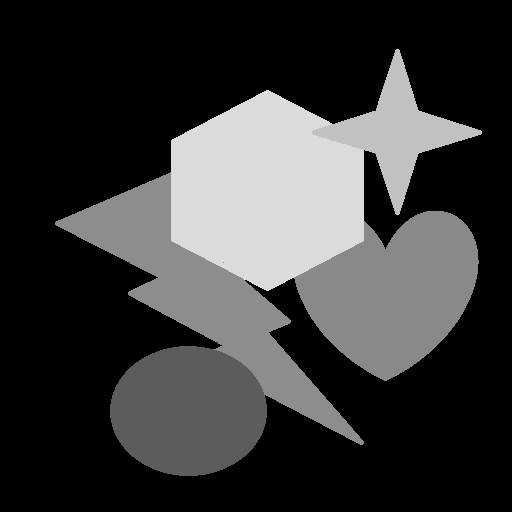
\includegraphics[width=14cm]{sample5}
    \end{figure}
    \newpage

    \begin{figure}[h!]
    \centering
    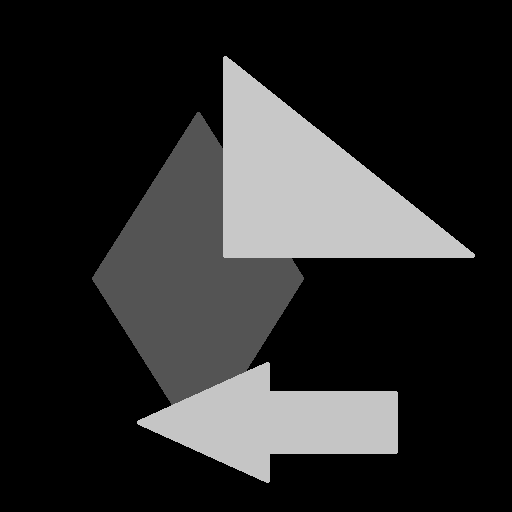
\includegraphics[width=14cm]{sample6}
    \end{figure}
    \newpage

    \begin{figure}[h!]
    \centering
    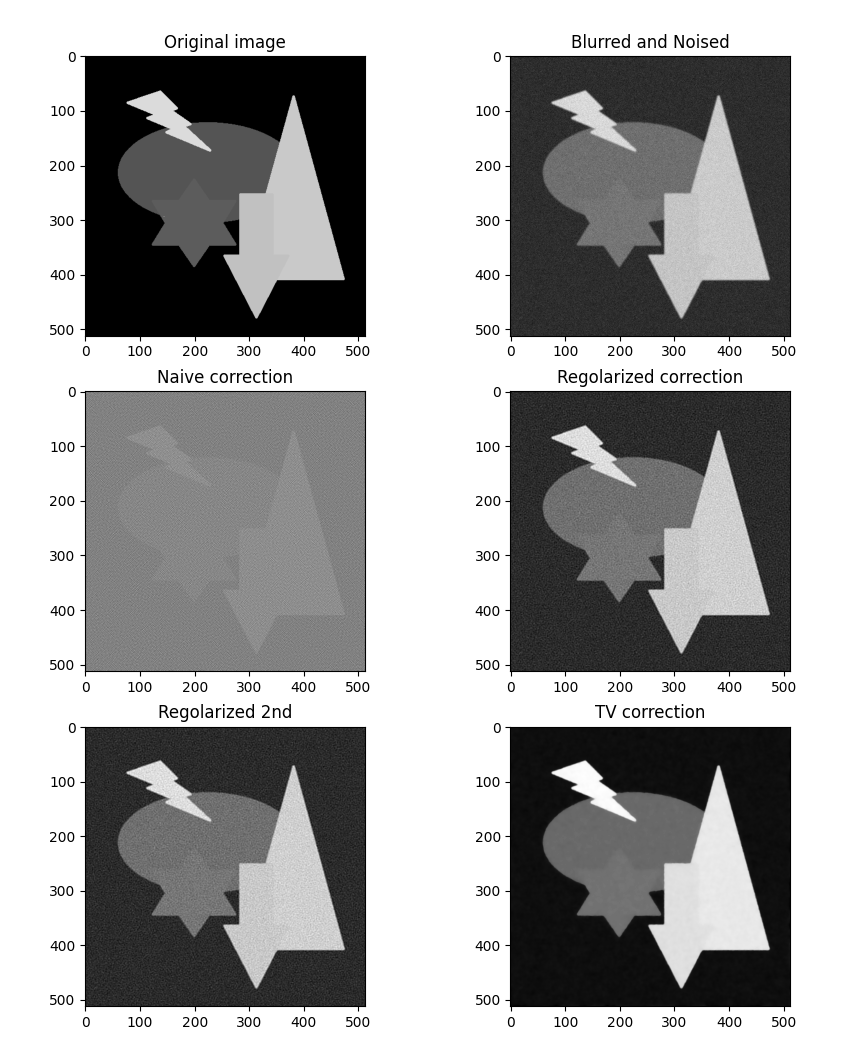
\includegraphics[width=14cm]{sample7}
    \end{figure}
    \newpage

    \begin{figure}[h!]
    \centering
    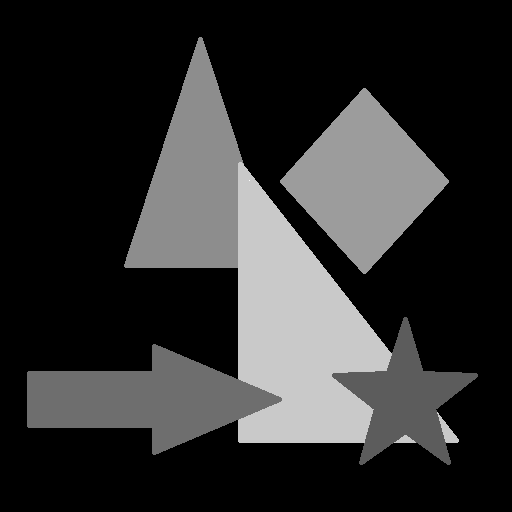
\includegraphics[width=14cm]{sample8}
    \end{figure}
    \newpage

    \begin{figure}[h!]
    \centering
    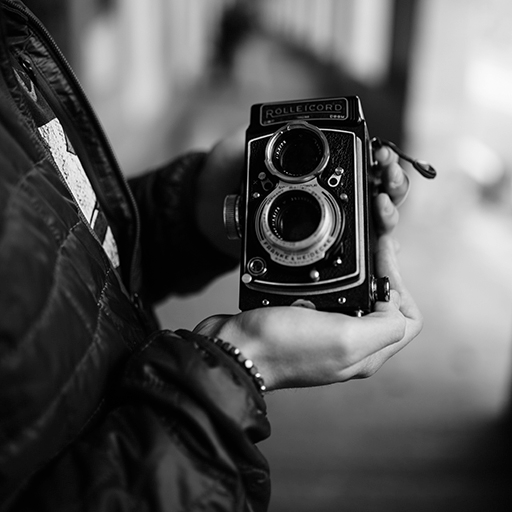
\includegraphics[width=14cm]{sample9}
    \end{figure}
    \newpage

    \begin{figure}[h!]
    \centering
    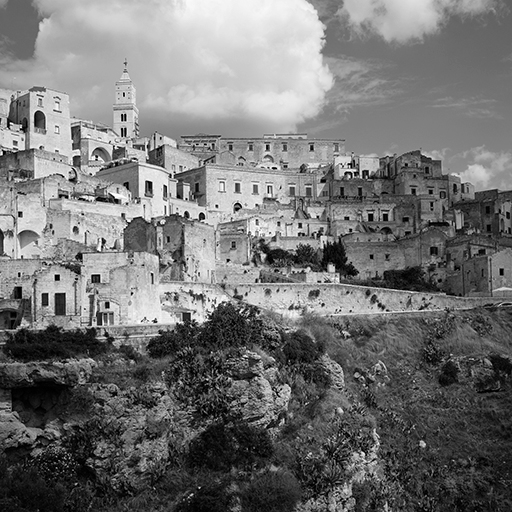
\includegraphics[width=14cm]{sample10}
    \end{figure}
    \newpage

\end{document}
